\chapter{One}
\section{Pictures}
Text before the first picture.
\begin{figure}[h]
\centering
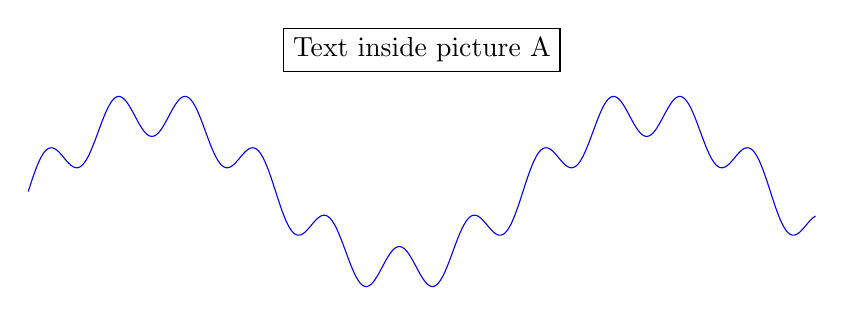
\begin{tikzpicture}
  \draw[domain=0:10,samples=3000,blue] plot (\x,{sin(\x r)+0.3*sin(7*\x r)});
  \node[draw] at (5,1.8) {Text inside picture A};
\end{tikzpicture}
\caption{A heavy plot}\label{fig:a}
\end{figure}
An inline picture \tikz \draw (0,0) circle (1ex); in a sentence, and one on a
baseline: 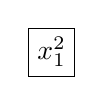
\begin{tikzpicture}[baseline=(n.base)]\node[draw](n){$x_1^2$};\end{tikzpicture}
continues.


\begin{tikzpicture}
  \node[draw] {See section~\ref{sec:two} on page~\pageref{sec:two}};
\end{tikzpicture}


\begin{tikzpicture}
  \node[draw] {This is page \thepage, figure \thefigure};
\end{tikzpicture}

Text with a \tikz[remember picture] \node (m) {mark}; and an overlay.
\begin{tikzpicture}[remember picture,overlay]
  \draw[->,red] (m) -- ++(2,1);
\end{tikzpicture}


\begin{tikzpicture}
  \node[draw] {\href{https://example.org}{a link in a picture}};
\end{tikzpicture}
